\subsection{Consuntivo complessivo}
\subsubsection{Consuntivo orario}
\begin{center}
	\renewcommand{\arraystretch}{1.8} %aumento ampiezza righe
	\begin{tabular}{ |m{8em}|c|c|c|c|c|c|c| }
	\hline
	\textbf{Membro} & \textbf{Re} & \textbf{Am} &  \textbf{An} &  \textbf{Pt} &  \textbf{Pg} &  \textbf{Ve} &  \textbf{Totale}\\
    \hline
    Irene Benetazzo   & 5 & 18 & 9  & 20 & 21 & 27 & \textbf{100} \\
    \hline
    Tommaso Berlaffa  & 4 & 10 & 15 & 24 & 27 & 20 & \textbf{100} \\
    \hline
    Mattia Episcopo   & 6 & 13 & 18 & 22 & 25 & 16 & \textbf{100} \\
    \hline
    Pietro Macrì      & 5 & 9  & 7  & 25 & 32 & 22 & \textbf{100} \\
    \hline
    Qi Fan Andrea Pan & 5 & 8  & 10 & 25 & 27 & 25 & \textbf{100} \\
    \hline
    Matteo Pillon     & 6 & 11 & 12 & 24 & 26 & 21 & \textbf{100} \\
    \hline
    Samuele Rizzato   & 9 & 16 & 14 & 20 & 22 & 19 & \textbf{100} \\
    \hline
    \textbf{Totale ore} & \textbf{40} & \textbf{85}  & \textbf{85} &  \textbf{160} &  \textbf{180} &  \textbf{150} &  \textbf{700}\\
    \hline
	\end{tabular}
\end{center}

\begin{figure}[H]
    \centering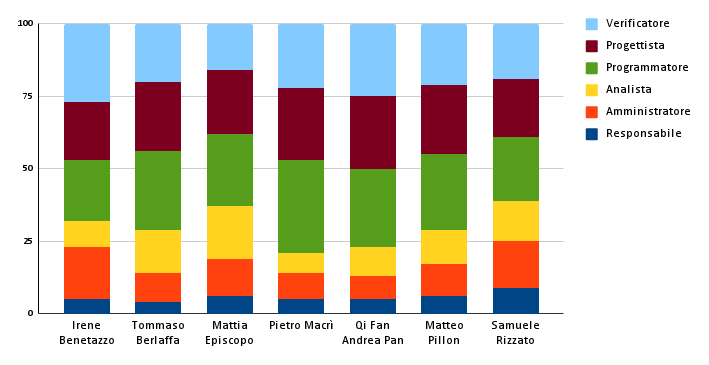
\includegraphics[width=\textwidth, height=\textheight,keepaspectratio]{images/consuntivo/Complessivo-orario.png}
    \caption{Consuntivo complessivo - consuntivo ripartizione oraria}
\end{figure}

\paragraph{Consuntivo Economico}
\begin{center}
	\renewcommand{\arraystretch}{1.8}
	\begin{tabular}{ |m{6em}|c|c|c|c|c|c|c| }
	\hline
	\textbf{Ruolo} & \textbf{Re} & \textbf{Am} &  \textbf{An} &  \textbf{Pt} &  \textbf{Pg} &  \textbf{Ve} &  \textbf{Totale}\\
    \hline
    Totale ore & 40 & 85 & 85 & 160 & 180 & 150 & \textbf{700}\\
    \hline
    Costo \euro/h & 30\euro/h & 20\euro/h & 25\euro/h & 25\euro/h & 15\euro/h & 15\euro/h & \\
    \hline
    \textbf{Totale costo} & \textbf{1200\euro} & \textbf{1700\euro} &  \textbf{2125\euro} & \textbf{4000\euro} &  \textbf{2700\euro} &  \textbf{2250\euro} &  \textbf{13975\euro} \\
    \hline
	\end{tabular}

    \begin{figure}[H]
        \centering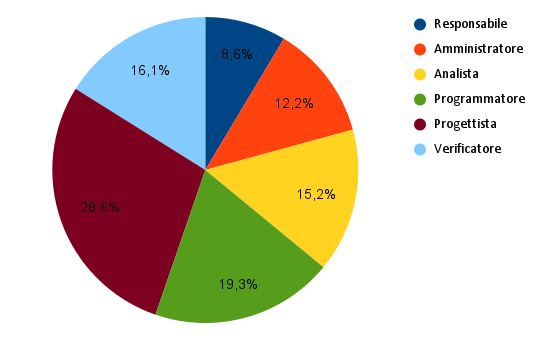
\includegraphics[width=0.7\textwidth, height=0.7\textheight, keepaspectratio]{images/consuntivo/Complessivo-costo.png}
        \caption{Consuntivo complessivo - consuntivo ripartizione economica}
    \end{figure}
\end{center}

\paragraph{Considerazioni} \hfill \break
Rispetto al preventivo presentato durante la candidatura ci sono stati diversi cambiamenti riguardo al numero di ore per i vari ruoli dettato dalla maggiore comprensione dei membri del gruppo riguardo le attività per il progetto. 
La pianificazione degli incrementi è variata rispetto a quanto preventivato per via dei ritardi dovuti allo studio di nuove tecnologie e alle tempistiche delle revisioni di avanzamento. 
Quindi sono stati implementati tutti i requisiti obbligatori, mentre solo alcuni dei desiderabili anche a causa di alcune risorse non ancora disponibili da parte dell'azienda.
\begin{center}
	\renewcommand{\arraystretch}{1.8}
	\begin{tabular}{ | l |c|c| }
    \hline
    & \textbf{Ore} & \textbf{Costo} \\
	\hline
    \textbf{Consuntivo complessivo} & 700 & 14200\euro \\
    \hline
    \textbf{Preventivo iniziale} & 700 & 13975\euro \\
    \hline
    \textbf{Bilancio} & - & -225\euro \\
    \hline
    \end{tabular}
\end{center}
Per preventivo iniziale si intende il preventivo dichiarato in fase di candidatura per l'aggiudicazione dell'appalto.
In conclusione questo progetto iniziato il 10 Aprile 2022 con l'assegnazione dell'appalto si conclude il 25 Settembre 2022 con 700 ore di lavoro totali e un costo complessivo di 13975€ quindi con un leggero risparmio economico rispetto al preventivo iniziale.